\clearpage
\onecolumn
\appendix
%\setcounter{page}{1}
%\maketitlesupplementary

\begin{center}
\vspace*{8pt}
\textbf{\Large ID-Consistent, Precise Expression Generation with Blendshape-Guided Diffusion}

\vspace{3pt}
\textbf{\Large (Supplementary Material)}
\vspace{20pt}
\end{center}

\section{Implementation Details}
\label{sec:implementation}

Our method builds on Arc2Face~\cite{paraperas2024arc2face}, which uses a fine-tuned UNet and ID encoder derived from \texttt{stable-diffusion-v1-5}. For our \textbf{Expression Adapter}, we employ a two-layer MLP, as well as separate identical key/value matrices into the UNet's cross-attention layers. Training is performed with AdamW~\cite{loshchilov2017decoupled} using a learning rate of 1e-4, a batch size of 8 per GPU, across 8 NVIDIA A100 GPUs for 300K iterations. For the \textbf{Reference Adapter}, we use a copy of Arc2Face’s UNet as the reference network and augment the original UNet with LoRA matrices of rank 128. The LoRA weights are trained using cross-paired frames from video datasets, as described in the main paper. We optimize them with a learning rate of 1e-5, using the same hardware configuration and a batch size of 8, for 15K iterations. For inference, we adopt DPM-Solver~\cite{lu2022dpm, lu2022dpm++} with 25 denoising steps and a classifier-free guidance scale of 3. For the LoRA weights in the \textbf{Reference Adapter}, we found a scale factor of 0.8 to provide a good balance between visual consistency with the input image and alignment with the target expression. Finally, for the baselines in our comparisons, we replace any additional text conditioning (if used by the method) with the prompt “photo of a person” to ensure a fair comparison that emphasizes identity and expression control.

\section{Additional Results}

Below, we provide additional visual comparisons in \cref{fig:comp_supp}, along with further generations from our \textbf{Expression Adapter} in \cref{fig:samples1,fig:samples2,fig:samples3}.

\begin{figure*}[h]
\centering
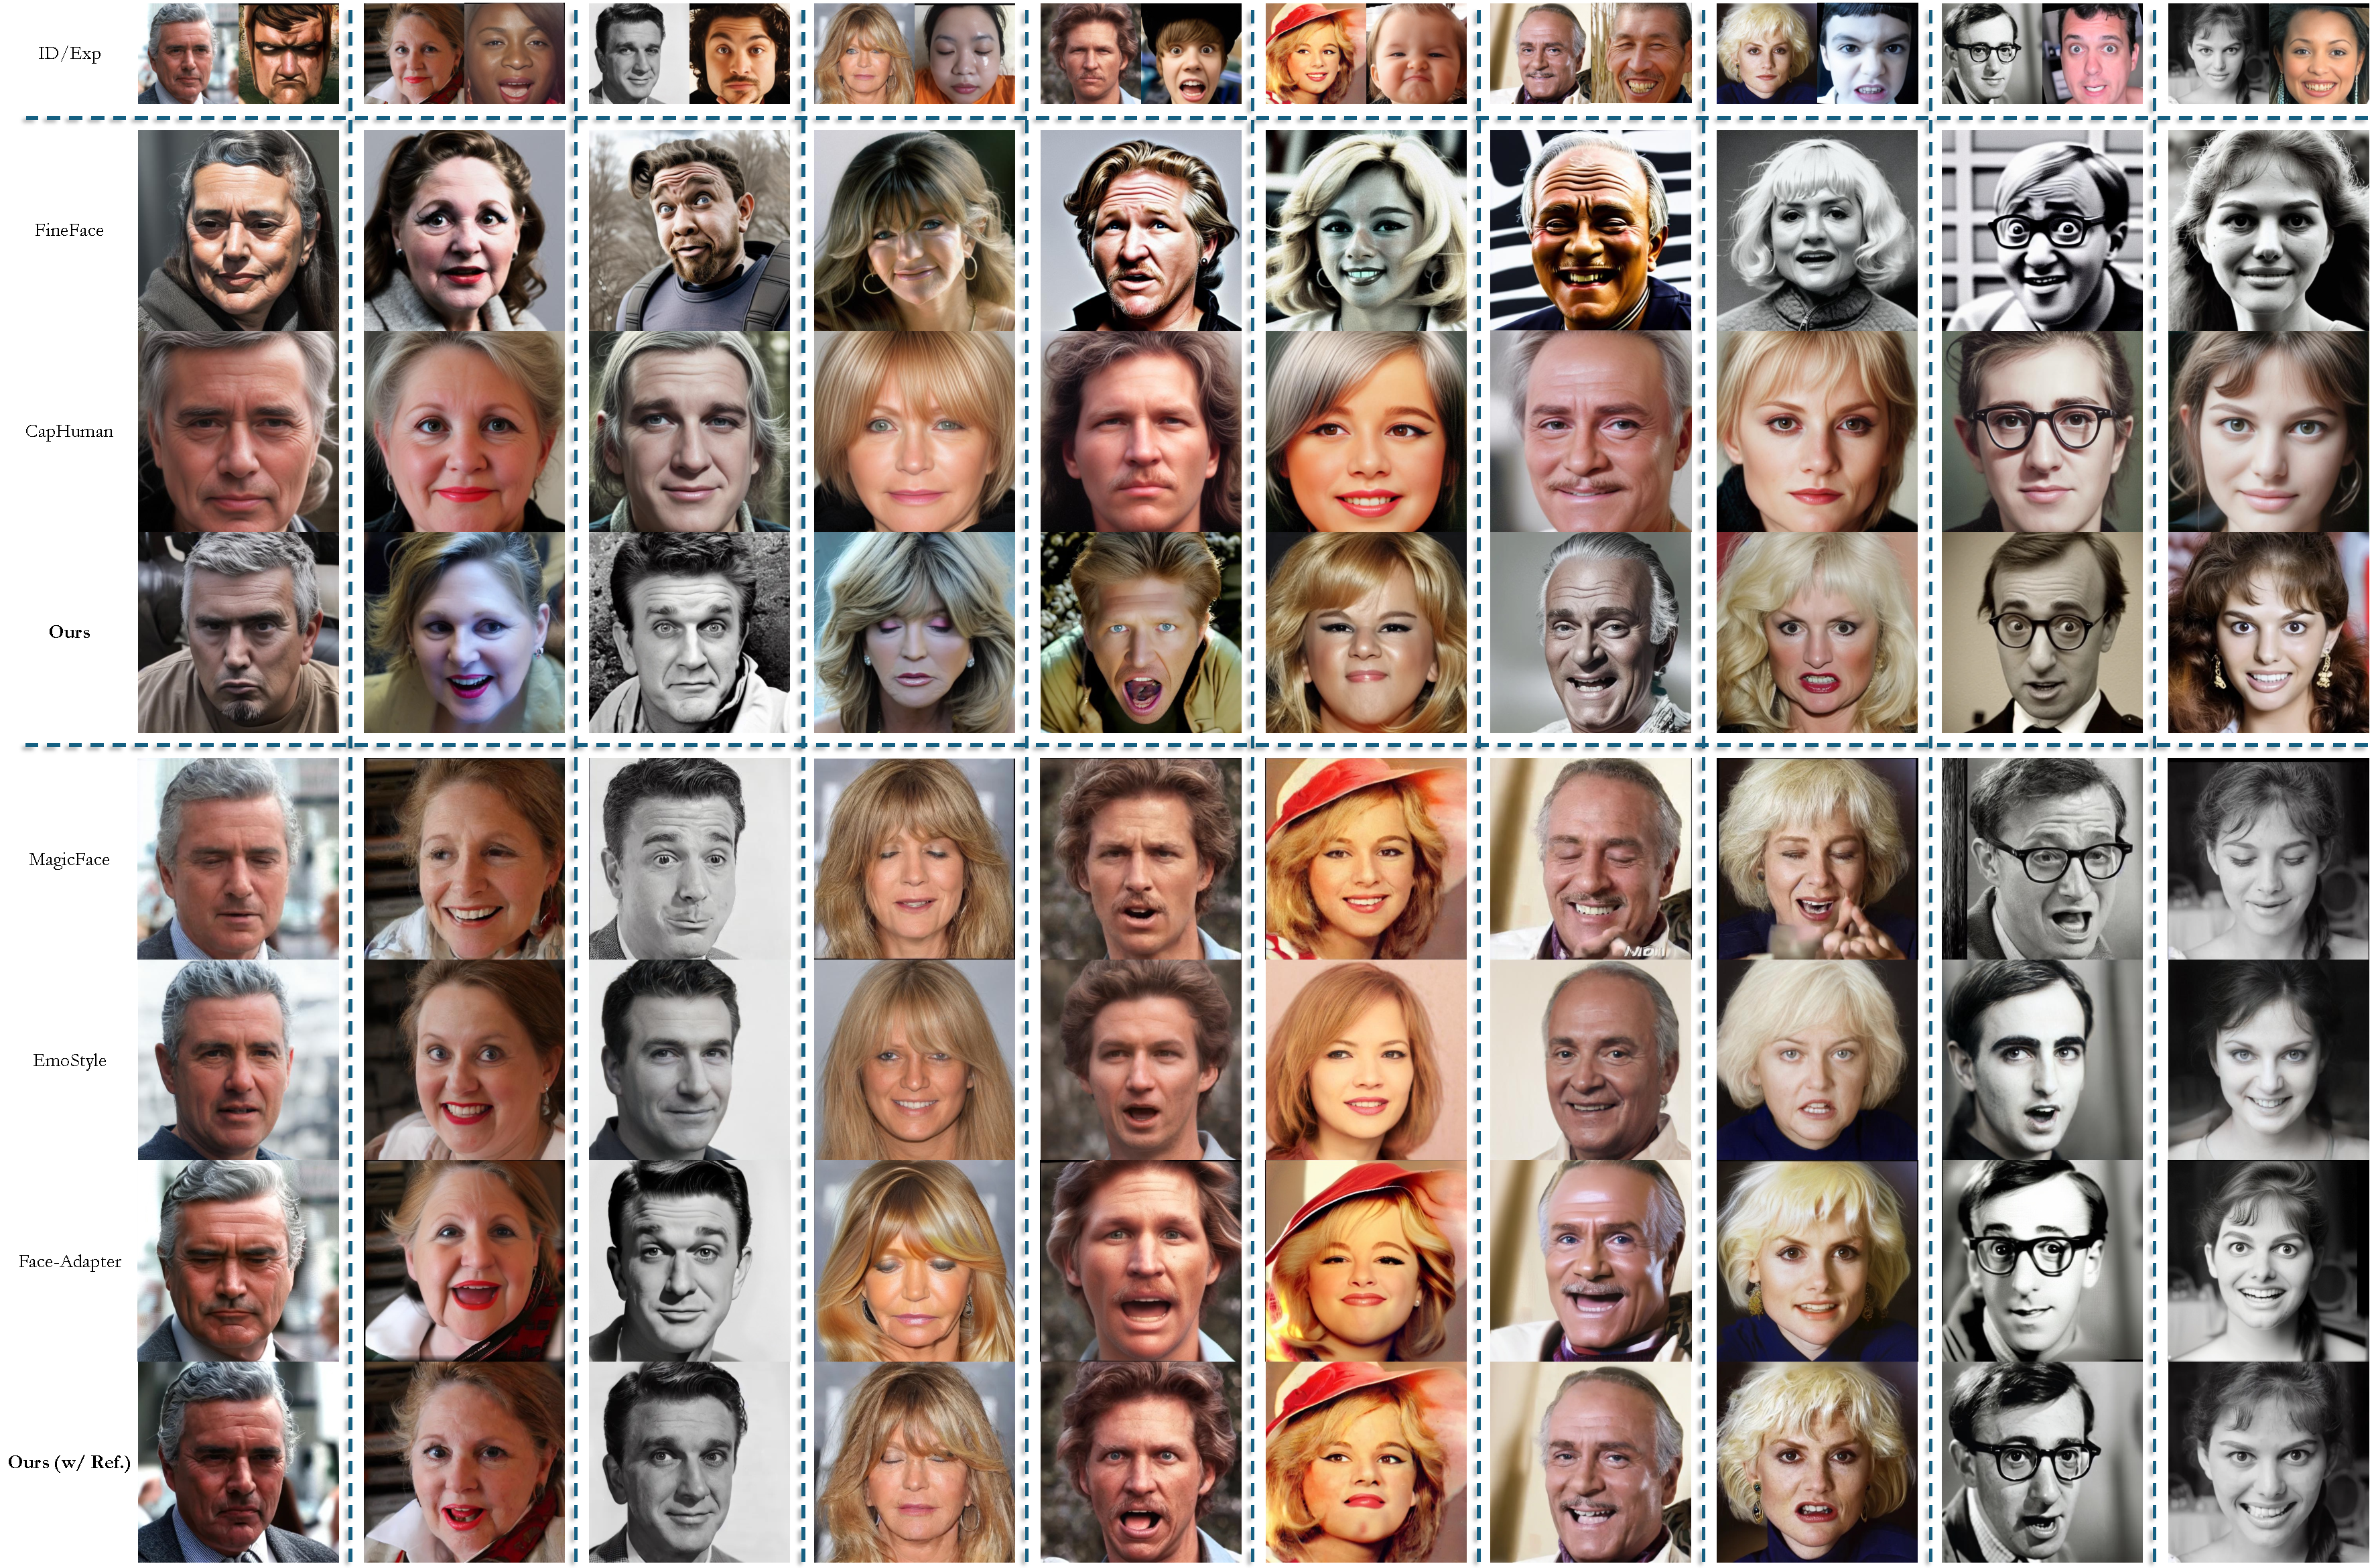
\includegraphics[width=0.87\textwidth]{figures/comp_supp.pdf}
\caption{Visual comparison between our method and competing expression-conditioned models. \textbf{Top:} ID-driven results compared to \cite{varanka2024fineface, liang2024caphuman}. \textbf{Bottom:} Reference-driven generation compared to \cite{wei2025magicface, azari2024emostyle, han2024faceadapter}. For the latter setting, our method is conditioned on both identity features and the reference image via the Reference Adapter.}
\label{fig:comp_supp}
\end{figure*}

\begin{figure*}[h]
\centering
\includegraphics[width=0.88\textwidth]{figures/samples1_compressed.pdf}
\caption{Samples generated by our model, conditioned on the input identity and the corresponding target expression.}
\label{fig:samples1}
\end{figure*}

\begin{figure*}[h]
\centering
\includegraphics[width=0.88\textwidth]{figures/samples2_compressed.pdf}
\caption{Samples generated by our model, conditioned on the input identity and the corresponding target expression (cont.).}
\label{fig:samples2}
\end{figure*}

\begin{figure*}[h]
\centering
\includegraphics[width=0.88\textwidth]{figures/samples3_compressed.pdf}
\caption{Samples generated by our model, conditioned on the input identity and the corresponding target expression (cont.).}
\label{fig:samples3}
\end{figure*}